\documentclass[12pt, a4paper, oneside]{ctexart}
\usepackage{amsmath, amsthm, amssymb, bm, color, graphicx, geometry, mathrsfs,extarrows, braket, booktabs, array, wrapfig, enumitem, subfigure, bbm}
\usepackage[colorlinks,linkcolor=red,anchorcolor=blue,citecolor=blue,urlcolor=blue,menucolor=black]{hyperref}
%%%% 设置中文字体 %%%%
% fc-list -f "%{family}\n" :lang=zh >d:zhfont.txt 命令查看已有字体
\setCJKmainfont[
    BoldFont=方正黑体_GBK,  % 黑体
    ItalicFont=方正楷体_GBK,  % 楷体
    BoldItalicFont=方正粗楷简体,  % 粗楷体
    Mapping = fullwidth-stop  % 将中文句号“.”全部转化为英文句号“.”,
]{方正书宋简体}  % !!! 注意在Windows中运行请改为“方正书宋简体.ttf” !!!
%%%% 设置英文字体 %%%%
\setmainfont{Minion Pro}
\setsansfont{Calibri}
\setmonofont{Fira Code}

%%%% 设置代码块 %%%%
% 在vscode中使用minted需要先配置python解释器, Ctrl+Shift+P, 输入Python: Select Interpreter选择安装了Pygments的Python版本. 再在setting.json中xelatex和pdflatex的参数中加入 "--shell-escape", 即可
% TeXworks中配置方法参考: https://blog.csdn.net/RobertChenGuangzhi/article/details/108140093
\usepackage{minted}
\renewcommand{\theFancyVerbLine}{
    \sffamily\textcolor[rgb]{0.5,0.5,0.5}{\scriptsize\arabic{FancyVerbLine}}} % 修改代码前序号大小
% 加入不同语言的代码块
\newmintinline{cpp}{fontsize=\small, linenos, breaklines, frame=lines}
\newminted{cpp}{fontsize=\small, baselinestretch=1, linenos, breaklines, frame=lines}
\newmintedfile{cpp}{fontsize=\small, baselinestretch=1, linenos, breaklines, frame=lines}
\newminted{r}{fontsize=\fontsize{10pt}{13pt}\selectfont, baselinestretch=1, linenos, breaklines, frame=lines}
\newmintedfile{r}{fontsize=\small, baselinestretch=1, linenos, breaklines, frame=lines}
\newmintinline{matlab}{fontsize=\small, linenos, breaklines, frame=lines}
\newminted{matlab}{fontsize=\small, baselinestretch=1, mathescape, linenos, breaklines, frame=lines}
\newmintedfile{matlab}{fontsize=\small, baselinestretch=1, linenos, breaklines, frame=lines}
\newmintinline{python}{fontsize=\small, linenos, breaklines, frame=lines, python3}  % 使用\pythoninline{代码}
\newminted{python}{fontsize=\small, baselinestretch=1, linenos, breaklines, frame=lines, python3}  % 使用\begin{pythoncode}代码\end{pythoncode}
\newmintedfile{python}{fontsize=\small, baselinestretch=1, linenos, breaklines, frame=lines, python3}  % 使用\pythonfile{代码地址}

%%%% 设置行间距与页边距 %%%%
\linespread{1.4}
%\geometry{left=2.54cm,right=2.54cm,top=3.18cm,bottom=3.18cm}
\geometry{left=1.84cm,right=1.84cm,top=2.18cm,bottom=2.18cm}

%%%% 图片相对路径 %%%%
\graphicspath{{figures/}} % 当前目录下的figures文件夹, {../figures/}则是父目录的figures文件夹
\setlength{\abovecaptionskip}{-0.2cm}  % 缩紧图片标题与图片之间的距离
\setlength{\belowcaptionskip}{0pt} 

%%%% 缩小item,enumerate,description两行间间距 %%%%
\setenumerate[1]{itemsep=0pt,partopsep=0pt,parsep=\parskip,topsep=5pt}
\setitemize[1]{itemsep=0pt,partopsep=0pt,parsep=\parskip,topsep=5pt}
\setdescription{itemsep=0pt,partopsep=0pt,parsep=\parskip,topsep=5pt}

%%%% 自定义公式 %%%%
\everymath{\displaystyle} % 默认全部行间公式
\DeclareMathOperator*\uplim{\overline{lim}} % 定义上极限 \uplim_{}
\DeclareMathOperator*\lowlim{\underline{lim}} % 定义下极限 \lowlim_{}
\DeclareMathOperator*{\argmax}{arg\,max}  % 定义取最大值的参数 \argmax_{}
\DeclareMathOperator*{\argmin}{arg\,min}  % 定义取最小值的参数 \argmin_{}
\let\leq=\leqslant % 将全部leq变为leqslant
\let\geq=\geqslant % geq同理
\DeclareRobustCommand{\rchi}{{\mathpalette\irchi\relax}}
\newcommand{\irchi}[2]{\raisebox{\depth}{$#1\chi$}} % 使用\rchi将\chi居中

%%%% 自定义环境配置 %%%%
\newcounter{problem}  % 问题序号计数器
\newenvironment{problem}[1][]{\stepcounter{problem}\par\noindent\textbf{题目\arabic{problem}. #1}}{\smallskip\par}
\newenvironment{solution}[1][]{\par\noindent\textbf{#1解答. }}{\smallskip\par}  % 可带一个参数表示题号\begin{solution}{题号}
\newenvironment{note}{\par\noindent\textbf{注记. }}{\smallskip\par}
\newenvironment{remark}{\begin{enumerate}[label=\textbf{注\arabic*.}]}{\end{enumerate}}
\BeforeBeginEnvironment{minted}{\vspace{-0.5cm}}  % 缩小minted环境距上文间距
\AfterEndEnvironment{minted}{\vspace{-0.2cm}}  % 缩小minted环境距下文间距

%%%% 一些宏定义 %%%%
\def\bd{\boldsymbol}        % 加粗(向量) boldsymbol
\def\disp{\displaystyle}    % 使用行间公式 displaystyle(默认)
\def\weekto{\rightharpoonup}% 右半箭头
\def\tsty{\textstyle}       % 使用行内公式 textstyle
\def\sign{\textrm{sign}}    % sign function
\def\cov{\textrm{Cov}}      % 
\def\var{\textrm{Var}}      % 
\def\E{\mathbb{E}}         % 
\def\T{\textrm{T}}          % 
\def\1{\bd{1}}
\def\wtd{\widetilde}        % 宽波浪线 widetilde
\def\R{\mathbb{R}}          % Real number
\def\N{\mathbb{N}}          % Natural number
\def\Z{\mathbb{Z}}          % Integer number
\def\Q{\mathbb{Q}}          % Rational number
\def\C{\mathbb{C}}          % Complex number
\def\K{\mathbb{K}}          % Number Field
\def\P{\textrm{P}}          % Possibility
\def\d{\mathrm{d}}          % differential operator
\def\e{\mathrm{e}}          % Euler's number
\def\i{\mathrm{i}}          % imaginary number
\def\re{\mathrm{Re}}        % Real part
\def\im{\mathrm{Im}}        % Imaginary part
\def\res{\mathrm{Res}}      % Residue
\def\ker{\mathrm{Ker}}      % Kernel
\def\vspan{\mathrm{vspan}}  % Span  \span与latex内核代码冲突改为\vspan
\def\L{\mathcal{L}}         % Loss function
\def\O{\mathcal{O}}         % big O notation
\def\wdh{\widehat}          % 宽帽子 widehat
\def\ol{\overline}          % 上横线 overline
\def\ul{\underline}         % 下横线 underline
\def\add{\vspace{1ex}}      % 增加行间距
\def\del{\vspace{-1.5ex}}   % 减少行间距

%%%% 定理类环境的定义 %%%%
\newtheorem{theorem}{定理}

%%%% 基本信息 %%%%
\newcommand{\RQ}{\today} % 日期
\newcommand{\km}{数据分析} % 科目
\newcommand{\bj}{强基数学002} % 班级
\newcommand{\xm}{吴天阳} % 姓名
\newcommand{\xh}{2204210460} % 学号

\begin{document}

%\pagestyle{empty}
\pagestyle{plain}
\vspace*{-15ex}
\centerline{\begin{tabular}{*5{c}}
    \parbox[t]{0.25\linewidth}{\begin{center}\textbf{日期}\\ \large \textcolor{blue}{\RQ}\end{center}} 
    & \parbox[t]{0.2\linewidth}{\begin{center}\textbf{科目}\\ \large \textcolor{blue}{\km}\end{center}}
    & \parbox[t]{0.2\linewidth}{\begin{center}\textbf{班级}\\ \large \textcolor{blue}{\bj}\end{center}}
    & \parbox[t]{0.1\linewidth}{\begin{center}\textbf{姓名}\\ \large \textcolor{blue}{\xm}\end{center}}
    & \parbox[t]{0.15\linewidth}{\begin{center}\textbf{学号}\\ \large \textcolor{blue}{\xh}\end{center}} \\ \hline
\end{tabular}}
\begin{center}
    \zihao{3}\textbf{第四次作业}
\end{center}\vspace{-0.2cm}
\begin{problem}[3.1]
    对于两因素等重复实验下的方差分析模型,证明下面四个等式成立:
    \begin{equation*}
        \sum_{i=1}^a\alpha_i= 0,\quad \sum_{j=1}^b\beta_j = 0,\quad\sum_{i=1}^a\gamma_{ij} = \sum_{j=1}^b\gamma_{ij} = 0.
    \end{equation*}
\end{problem}\vspace*{-1cm}
\begin{proof}
    由于
    \begin{align*}
        &\ \mu = \frac{1}{ab}\sum_{\substack{1\leq i\leq a\\1\leq j\leq b}}\mu_{ij},\quad \mu_{i\cdot}=\frac{1}{b}\sum_{j=1}^n\mu_{ij},\quad \alpha_i = \mu_{i\cdot}-\mu\\
        &\ \mu_{\cdot j} = \frac{1}{a}\sum_{i=1}^a\mu_{ij},\quad \beta_j = \mu_{\cdot j} - \mu,\quad \gamma_{ij} = (\mu_{ij} - \mu)-(\alpha_i+\beta_j)
    \end{align*}
    于是
    \begin{align*}
        \sum_{i=1}^a\alpha_i =&\ \sum_{i=1}^a\mu_{i\cdot}-a\mu = \frac{1}{b}\sum_{\substack{1\leq i\leq a\\ 1\leq j \leq b}}\mu_{ij} - \frac{1}{b}\sum_{\substack{1\leq i\leq a\\ 1\leq j \leq b}}\mu_{ij} = 0\\
        \sum_{j=1}^b\beta_j =&\ \sum_{j=1}^b\mu_{\cdot j}-b\mu = \frac{1}{a}\sum_{\substack{1\leq i\leq a\\ 1\leq j \leq b}}\mu_{ij} - \frac{1}{a}\sum_{\substack{1\leq i\leq a\\ 1\leq j \leq b}}\mu_{ij} = 0\\
        \sum_{i=1}^a\gamma_{ij} =&\ \sum_{i=1}^a\mu_{ij}-a\mu-\left(\sum_{i=1}^a\alpha_{i}+a\beta_{j}\right) = a(\mu_{\cdot j} - \mu)-a(\mu_{\cdot j}-\mu) = 0\\
        \sum_{i=1}^b\gamma_{ij} =&\ \sum_{i=1}^b\mu_{ij}-b\mu-\left(b\alpha_{i}+\sum_{j=1}^b\beta_{j}\right) = b(\mu_{i\cdot} - \mu)-b(\mu_{i\cdot}-\mu) = 0
    \end{align*}
\end{proof}
\begin{problem}
    对方差分析模型推导
    \begin{equation*}
    \begin{cases}
        \E(SS_A) = (a-1)\sigma^2 + bc\sum_{i=1}^a\alpha_i^2,\\
        \E(SS_B) = (b-1)\sigma^2 + bc\sum_{i=1}^b\beta_j^2,\\
        \E(SS_{AB}) = (a-1)(b-1)\sigma^2 + c\sum_{i=1}^a\sum_{j=1}^b\gamma_{ij}^2,\\
        \E(SS_E) = ab(c-1)\sigma^2.
    \end{cases}
    \end{equation*}
\end{problem}
\begin{proof}
    由于$\E(\bar{\varepsilon}_{i\cdot\cdot}) = \E(\bar{\varepsilon}) = 0,\ \E\left[\frac{1}{a-1}\sum_{i=1}^a(\bar{\varepsilon}_{i\cdot\cdot}-\bar{\varepsilon})^2\right] = \frac{\sigma^2}{bc}$,于是
    \begin{align*}
        \E(SS_A) =&\ \E\left[bc\sum_{i=1}^a(\alpha_i+\bar{\varepsilon}_{i\cdot\cdot}-\bar{\varepsilon})^2\right]\\
        =&\ bc \sum_{i=1}^a\alpha_i^2 + 2bc\sum_{i=1}^a\alpha_i(\bar{\varepsilon}_{i\cdot\cdot}-\bar{\varepsilon})+bc\sum_{i=1}^a(\bar{\varepsilon}_{i\cdot\cdot}-\bar{\varepsilon})^2\\
        =&\ bc\sum_{i=1}^a\alpha_i^2+(a-1)bc\cdot\frac{\sigma^2}{bc} = (a-1)\sigma^2+bc\sum_{i=1}^a\alpha_i^2
    \end{align*}
    
    由于$\E(\bar{\varepsilon}_{\cdot j\cdot}) = \E(\bar{\varepsilon}) = 0,\ \E\left[\frac{1}{b-1}\sum_{j=1}^b(\bar{\varepsilon}_{\cdot j\cdot}-\bar{\varepsilon})^2\right] = \frac{\sigma^2}{ac}$,于是
    \begin{align*}
        \E(SS_B) =&\ \E\left[ac\sum_{j=1}^b(\beta_j+\bar{\varepsilon}_{\cdot j\cdot}-\bar{\varepsilon})^2\right]\\
        =&\ ac \sum_{j=1}^b\beta_j^2 + 2ac\sum_{j=1}^b\beta_j(\bar{\varepsilon}_{\cdot j\cdot}-\bar{\varepsilon})+bc\sum_{j=1}^b(\bar{\varepsilon}_{\cdot j\cdot}-\bar{\varepsilon})^2\\
        =&\ ac\sum_{j=1}^b\beta_j^2+(b-1)ac\cdot\frac{\sigma^2}{ac} = (b-1)\sigma^2+ac\sum_{j=1}^b\beta_j^2
    \end{align*}
    由于$\E(\bar{\varepsilon}_{ij\cdot}) = 0,\ \E\left[\frac{1}{(a-1)(b-1)}\sum_{\substack{1\leq i\leq a\\1\leq j\leq b}}(\bar{\varepsilon}_{ij\cdot}-\bar{\varepsilon}_{i\cdot\cdot}-\bar{\varepsilon}_{\cdot j\cdot}+\bar{\varepsilon})^2\right] = \frac{\sigma^2}{c}$,于是
    \begin{align*}
        \E(SS_{AB})=&\ \E\left[c\sum_{\substack{1\leq i\leq a\\1\leq j\leq b}}(\gamma_{ij}+\bar{\varepsilon}_{ij\cdot}-\bar{\varepsilon}_{i\cdot\cdot}-\bar{\varepsilon}_{\cdot j\cdot}+\bar{\varepsilon})^2\right]\\
        =&\ c\sum_{\substack{1\leq i\leq a\\1\leq j\leq b}}\gamma_{ij}^2+\E\left[2c\sum_{\substack{1\leq i\leq a\\1\leq j\leq b}}\gamma_{ij}(\bar{\varepsilon}_{ij\cdot}-\bar{\varepsilon}_{i\cdot\cdot}-\bar{\varepsilon}_{\cdot j\cdot}+\bar{\varepsilon})+c\sum_{\substack{1\leq i\leq a\\1\leq j\leq b}}(\bar{\varepsilon}_{ij\cdot}-\bar{\varepsilon}_{i\cdot\cdot}-\bar{\varepsilon}_{\cdot j\cdot}+\bar{\varepsilon})^2\right]\\
        =&\ c\sum_{\substack{1\leq i\leq a\\1\leq j\leq b}}\gamma_{ij}^2+c(a-1)(b-1)\frac{\sigma^2}{c}
        = c\sum_{\substack{1\leq i\leq a\\1\leq j\leq b}}\gamma_{ij}^2+(a-1)(b-1)\sigma^2
    \end{align*}
    由于$\E\left[\frac{1}{ab(c-1)}\sum_{i=1}^a\sum_{j=1}^b\sum_{k=1}^c(\varepsilon_{ijk}-\bar{\varepsilon}_{ij\cdot})^2\right] = \frac{\sigma^2}{ab(c-1)}$,于是
    \begin{equation*}
        \E(SS_E) = \E\left[\sum_{i=1}^a\sum_{j=1}^b\sum_{k=1}^c(\varepsilon_{ijk} - \bar{\varepsilon}_{ij\cdot})^2\right] = ab(c-1)\sigma^2.
    \end{equation*}
\end{proof}
\begin{problem}[3.5]
    为研究生产某种电子设备的公司在过去三年中的科研经费投入(分为低、中、高三档)对当年生产能力提高的影响,调查了总共27家生产该设备的公司,对当年生产能力与之三年前的提高量作评估,数据如书上表3.16所示,假定生产能力提高量服从方差分析模型。

    (1) 建立方差分析表,在显著水平$\alpha=0.05$下检验过去三年科研经费投入的不同是否对当年生产力的提高有显著性影响。

    (2) 分别以$\mu_L,\mu_M$和$\mu_H$记在过去三年科研经费投入为低、中、高情况下当年生产能力提高量的均值,分别给出$\mu_L,\mu_M$和$\mu_H$的置信度为$95\%$的置信区间以及差值$\mu_L-\mu_M,\mu_L-\mu_H$和$\mu_M-\mu_H$的置信度不小于$95\%$的Bonferroni同时置信区间。
    是否过去三年科研经费投入越高,当年生产能力的改善越显著?
\end{problem}
\begin{solution}
    (1)
    \begin{rcode}
> data <- data.frame(
  improvement = c(7.6, 8.2, 6.8, 5.8, 6.9, 6.6, 6.3, 7.7, 6.0,
  6.7, 8.1, 9.4, 8.6, 7.8, 7.7, 8.9, 7.9, 8.3, 8.7, 7.1, 8.4,
  8.5, 9.7, 10.1, 7.8, 9.6, 9.5),
  funding = factor(c(rep("low", 9), rep("medium", 12), rep("high", 6)))
)
fit <- aov(improvement ~ funding, data = data)
> summary(fit)
            Df Sum Sq Mean Sq F value   Pr(>F)    
funding      2  20.12   10.06   15.72 4.33e-05 ***
Residuals   24  15.36    0.64                     
---
Signif. codes:  0 ‘***’ 0.001 ‘**’ 0.01 ‘*’ 0.05 ‘.’ 0.1 ‘ ’ 1
    \end{rcode}
    上面代码中的输出给出了方差分析表,从该表中可以看出科研经费投入的因子$p$值为$4.33\times 10^{-5}$远小于$0.05$,所以拒绝原假设,
    认为过去三年科研经费投入的不同对当年生产力的提高有显著性影响。

    上表中其他信息分别表明\texttt{Df}为自由度,\texttt{Sum Sq}为平方和,\texttt{Mean Sq}为均方,\texttt{F value}为F统计量。

    (2)
    \begin{rcode}
> group_means <- tapply(data$improvement, data$funding, mean)
group_se <- tapply(data$improvement, data$funding, function(x) sd(x) / sqrt(length(x)))
group_df <- tapply(data$improvement, data$funding, function(x) length(x) - 1)

ci_low <- group_means - qt(0.975, group_df) * group_se
ci_high <- group_means + qt(0.975, group_df) * group_se

data.frame(
  funding = names(group_means),
  mean = group_means,
  ci_low = ci_low,
  ci_high = ci_high
)


       funding     mean   ci_low   ci_high
high      high 9.200000 8.289951 10.110049
low        low 6.877778 6.252390  7.503166
medium  medium 8.133333 7.652239  8.614427
    \end{rcode}
    上面代码结果说明$\mu_L,\mu_M,\mu_H$的$95\%$置信区间分别为$[6.3,7.5],[7.7,8.6],[8.3,10.1]$。
    \begin{rcode}
> t.test(data$improvement ~ data$funding, subset = data$funding %in% c("low", "medium"), conf.level = 0.95/3)
confidence interval: -1.400159 -1.110952
> t.test(data$improvement ~ data$funding, subset = data$funding %in% c("low", "high"), conf.level = 0.95/3)
confidence interval: -2.509356 -2.135088 
> t.test(data$improvement ~ data$funding, subset = data$funding %in% c("medium", "high"), conf.level = 0.95/3)
confidence interval: -1.2420397 -0.8912936 
    \end{rcode}
    上面结果说明$\mu_L-\mu_M,\mu_L-\mu_H,\mu_M-\mu_H$的不小于$95\%$的置信区间分别为$[-1.4,-1.1]$, $[-2.5,-2.1]$, $[-1.2,-0.9]$,
    所以可以认为过去三年的科研经费投入越高,当年的生产能力改善越显著。
\end{solution}
\begin{problem}[3.6]
    将小白鼠分为6组,其中三组分别给三种不同剂量(高、中、低)的三价铁,另三组给相应剂量的二价铁,数据如书上表$3.17$所示.

    (1). 求出个组合水平上的观测值的样本均值和标准差。各水平组合上的标准差(从而样本方差)差异是否明显?假定误差的等方差性是否合理?

    (2) 对观测数据作自然对数变换,再进行(1)中的分析,此时,各组合水平上的标准差是否趋于一致?

    (3) 对变换后的数据进行方差分析,建立方差分析表。在显著水平$\alpha=0.05$下,因素的交互相应是否显著?各因素的影响是否显著?

    (4) 根据(3)中分析,分别求各因素在其不同水平上的均值的置信度为$95\%$的置信区间以及两两均值之差的置信度不小于$95\%$的Bonferroni同时置信区间,并解释其结果。
\end{problem}
\begin{solution}
    (1)\begin{rcode}
> data <- read.csv("/home/wty/Documents/LaTex-Projects/Data Analysis/10,11,12,13/3.6.csv", skip = 2, header = FALSE)
> means <- colMeans(data)                                                                                           
sds <- apply(data, 2, sd)
> means
       V1        V2        V3        V4        V5        V6 
 3.698889  8.203889 11.750000  5.936667  9.632222 12.639444 
> sds
      V1       V2       V3       V4       V5       V6 
2.030870 5.447386 7.028150 2.806778 6.691215 6.082089 
    \end{rcode}
    样本方差差异较为明显,假定等方差性不合理。

    (2) \begin{rcode}
> data_log <- log(data)
means_log <- colMeans(data_log)
sds_log <- apply(data_log, 2, sd)
> means_log
        V1       V2       V3       V4       V5       V6 
1.160924 1.901225 2.279981 1.680129 2.090045 2.403389 
> sds_log
        V1        V2        V3        V4        V5        V6 
0.5854773 0.6585116 0.6563113 0.4645464 0.5736511 0.5693701 
    \end{rcode}
    标准差现在能够趋于一致。

    (3). \begin{rcode}
colnames(data_log) <- c("Fe3+_High", "Fe3+_Mid", "Fe3+_Low", "Fe2+_High", "Fe2+_Mid", "Fe2+_Low")
data_long <- gather(data_log, key = "group_dose", value = "value")
data_long_sep <- separate(data_long, group_dose, into = c("Fe", "dose"), sep = "_")
> fit <- aov(value ~ Fe * dose, data = data_long_sep)
summary(fit)
                Df Sum Sq Mean Sq F value   Pr(>F)    
Fe            1   2.07   2.074   5.993   0.0161 *  
dose          2  15.59   7.794  22.524 7.91e-09 ***
Fe:dose       2   0.81   0.405   1.171   0.3143    
Residuals   102  35.30   0.346                     
---
Signif. codes:  0 ‘***’ 0.001 ‘**’ 0.01 ‘*’ 0.05 ‘.’ 0.1 ‘ ’ 1
    \end{rcode}
    在显著性水平为$0.05$下,铁离子\texttt{Fe}和剂量\texttt{dose}之间的交互效应检验$p$值为$0.3143$大于$0.05$,所以交互效应不显著;
    而各因素的检验p值都是小于$0.05$的,所以各因素的影响是显著的。

    (4). \begin{rcode}
> TukeyHSD(fit)
Tukey multiple comparisons of means
    95% family-wise confidence level

Fit: aov(formula = value ~ Fe * dose, data = data_long_sep)

$Fe
                diff        lwr         upr     p adj
Fe3+-Fe2+ -0.2771441 -0.5016931 -0.05259515 0.0160691

$dose
                diff        lwr         upr     p adj
Low-High  0.9211588  0.5913881  1.25092946 0.0000000
Mid-High  0.5751084  0.2453377  0.90487914 0.0002042
Mid-Low  -0.3460503 -0.6758210 -0.01627962 0.0373939

$`Fe:dose`
                        diff         lwr        upr     p adj
Fe3+:High-Fe2+:High -0.5192055 -1.08875196 0.05034103 0.0952634
Fe2+:Low-Fe2+:High   0.7232596  0.15371311 1.29280610 0.0047746
Fe3+:Low-Fe2+:High   0.5998524  0.03030595 1.16939894 0.0328600
Fe2+:Mid-Fe2+:High   0.4099156 -0.15963091 0.97946208 0.3004966
Fe3+:Mid-Fe2+:High   0.2210958 -0.34845067 0.79064233 0.8688323
Fe2+:Low-Fe3+:High   1.2424651  0.67291857 1.81201157 0.0000001
Fe3+:Low-Fe3+:High   1.1190579  0.54951141 1.68860441 0.0000017
Fe2+:Mid-Fe3+:High   0.9291210  0.35957455 1.49866755 0.0001005
Fe3+:Mid-Fe3+:High   0.7403013  0.17075480 1.30984779 0.0035672
Fe3+:Low-Fe2+:Low   -0.1234072 -0.69295366 0.44613934 0.9885742
Fe2+:Mid-Fe2+:Low   -0.3133440 -0.88289052 0.25620248 0.6017585
Fe3+:Mid-Fe2+:Low   -0.5021638 -1.07171027 0.06738272 0.1166473
Fe2+:Mid-Fe3+:Low   -0.1899369 -0.75948336 0.37960964 0.9267813
Fe3+:Mid-Fe3+:Low   -0.3787566 -0.94830312 0.19078988 0.3891760
Fe3+:Mid-Fe2+:Mid   -0.1888198 -0.75836625 0.38072674 0.9284873

    \end{rcode}
对于Fe因素,$\text{Fe}^{3+}$和$\text{Fe}^{2+}$两个水平之间的均值差为$-0.277$,置信区间为$(-0.502, -0.053)$,$p$值为$0.016$。
说明在显著水平$\alpha=0.05$下,$\text{Fe}^{3+}$和$\text{Fe}^{2+}$两个水平之间的均值差异是显著的。

对于剂量因素,各水平之间的均值差异都是显著的($p$值均小于$0.05$)。
\end{solution}
\begin{problem}[3.7]
    将两种成分$A,B$按照三种不同剂量(低、中、高)混合,将受试患者分为9组,每组4人服用混合药物,记录病情缓解时间,如书上表3.18所示。

    (1) 计算每个水平组合($A_i,B_j$)上的均值$\mu_{ij}$的估计值$\bar{y}_{ij\cdot}(i,j=1,2,3)$,做出形如图3.2的图形(各水平组合为x轴,$\bar{y}_{ij\cdot}$为y轴的两个图像),判断$A$与$B$的交互效应是否显著。

    (2) 假设所给的数据服从方差分析模型,建立方差分析表,$A$与$B$的交互效应在显著性水平$\alpha=0.05$下是否显著?

    (3) 若$A$与$B$的交互效应显著,分别就$A$的各水平$A_i(i=1,2,3)$,给出在$B$的各水平$B_j$上的均值$\mu_{ij}$的置信度为$95\%$的置信区间以及两两之差的置信度不小于$95\%$的Bonferroni同时置信区间。
    固定$B$的各水平$B_j$,关于因素$A$作类似分析,能否选出最佳的水平组合?
\end{problem}
\begin{solution}
    (1)\begin{rcode}
data <- data.frame(
    A = rep(c("低剂量", "中剂量", "高剂量"), each = 12),
    B = rep(rep(c("低剂量", "中剂量", "高剂量"), each = 4), 3),
    value = c(2.4,2.7,2.3,2.5,4.6,4.2,4.9,4.7,4.8,4.5,4.4,4.6,
                5.8,5.2,5.5,5.3,8.9,9.1,8.7,9,9.1,9.3,8.7,9.4,
                6.1,5.7,5.9,6.2,9.9,10.5,10.6,10.1,13.5,13.0,
                13.3,13.2)
    )
# 使用dplyr包来计算每个水平组合的均值 
library(dplyr)
data_summary <- data %>%
group_by(A,B) %>%
summarise(mean_value = mean(value))
# 使用ggplot2包来绘制图形
library(ggplot2)
myplot <- ggplot(data_summary,aes(x=B,y=mean_value,color=A)) +
geom_point() +
geom_line() +
facet_wrap(~A) +
labs(title="各组和水平上的样本均值",x="成分B",y="均值")
print(myplot)
    \end{rcode}
\begin{figure}[htbp]
    \centering
    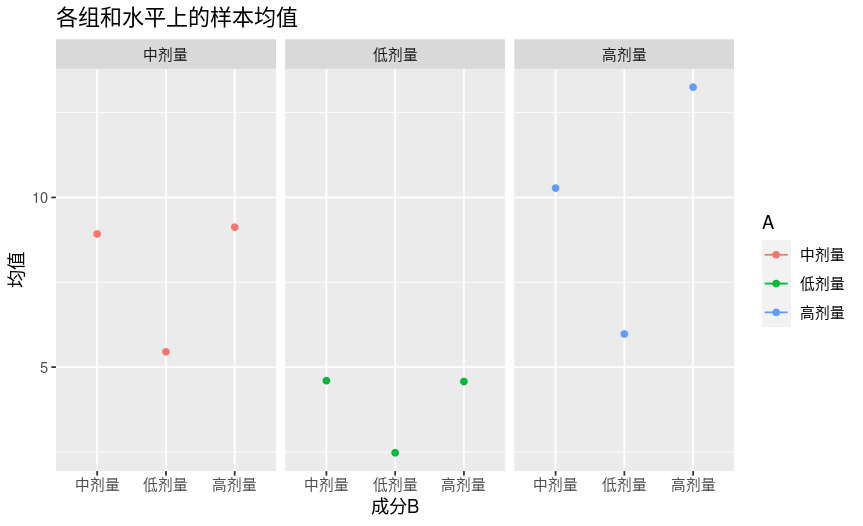
\includegraphics[scale=0.8]{3.7.png}
\end{figure}
如下图所示,从图中可以看出$A$与$B$的交互效应显著。

    (2)\begin{rcode}
> fit <- aov(value ~ A * B, data = data)
> summary(fit)
            Df Sum Sq Mean Sq F value Pr(>F)    
A            2 220.02  110.01  1827.9 <2e-16 ***
B            2 123.66   61.83  1027.3 <2e-16 ***
A:B          4  29.42    7.36   122.2 <2e-16 ***
Residuals   27   1.63    0.06                   
---
Signif. codes:  0 ‘***’ 0.001 ‘**’ 0.01 ‘*’ 0.05 ‘.’ 0.1 ‘ ’ 1 
    \end{rcode}
    由于\texttt{A:B}的交互相应的$p$值远小于$0.05$,所以可以认为交互效应显著。

    (3) \begin{rcode}
> data %>%
+     group_by(A,B) %>%
+     summarise(t.test(value)$conf.int)
   A      B      `t.test(value)$conf.int`
   <chr>  <chr>                     <dbl>
 1 中剂量 中剂量                     8.65
 2 中剂量 中剂量                     9.20
 3 中剂量 低剂量                     5.03
 4 中剂量 低剂量                     5.87
 5 中剂量 高剂量                     8.63
 6 中剂量 高剂量                     9.62
 7 低剂量 中剂量                     4.13
 8 低剂量 中剂量                     5.07
 9 低剂量 低剂量                     2.20
10 低剂量 低剂量                     2.75
11 低剂量 高剂量                     4.30
12 低剂量 高剂量                     4.85
13 高剂量 中剂量                     9.75
14 高剂量 中剂量                    10.8 
15 高剂量 低剂量                     5.62
16 高剂量 低剂量                     6.33
17 高剂量 高剂量                    12.9 
18 高剂量 高剂量                    13.6 

> TukeyHSD(fit)
Tukey multiple comparisons of means
    95% family-wise confidence level

Fit: aov(formula = value ~ A * B, data = data)

$A
                diff       lwr       upr p adj
低剂量-中剂量 -3.95 -4.198324 -3.701676     0
高剂量-中剂量  2.00  1.751676  2.248324     0
高剂量-低剂量  5.95  5.701676  6.198324     0

$B
                diff        lwr       upr p adj
低剂量-中剂量 -3.30 -3.5483241 -3.051676     0
高剂量-中剂量  1.05  0.8016759  1.298324     0
高剂量-低剂量  4.35  4.1016759  4.598324     0

$`A:B`
                            diff        lwr        upr     p adj
低剂量:中剂量-中剂量:中剂量 -4.325 -4.9086813 -3.7413187 0.0000000
高剂量:中剂量-中剂量:中剂量  1.350  0.7663187  1.9336813 0.0000007
中剂量:低剂量-中剂量:中剂量 -3.475 -4.0586813 -2.8913187 0.0000000
低剂量:低剂量-中剂量:中剂量 -6.450 -7.0336813 -5.8663187 0.0000000
高剂量:低剂量-中剂量:中剂量 -2.950 -3.5336813 -2.3663187 0.0000000
中剂量:高剂量-中剂量:中剂量  0.200 -0.3836813  0.7836813 0.9596929
低剂量:高剂量-中剂量:中剂量 -4.350 -4.9336813 -3.7663187 0.0000000
高剂量:高剂量-中剂量:中剂量  4.325  3.7413187  4.9086813 0.0000000
高剂量:中剂量-低剂量:中剂量  5.675  5.0913187  6.2586813 0.0000000
中剂量:低剂量-低剂量:中剂量  0.850  0.2663187  1.4336813 0.0011424
低剂量:低剂量-低剂量:中剂量 -2.125 -2.7086813 -1.5413187 0.0000000
高剂量:低剂量-低剂量:中剂量  1.375  0.7913187  1.9586813 0.0000005
中剂量:高剂量-低剂量:中剂量  4.525  3.9413187  5.1086813 0.0000000
低剂量:高剂量-低剂量:中剂量 -0.025 -0.6086813  0.5586813 1.0000000
高剂量:高剂量-低剂量:中剂量  8.650  8.0663187  9.2336813 0.0000000
中剂量:低剂量-高剂量:中剂量 -4.825 -5.4086813 -4.2413187 0.0000000
低剂量:低剂量-高剂量:中剂量 -7.800 -8.3836813 -7.2163187 0.0000000
高剂量:低剂量-高剂量:中剂量 -4.300 -4.8836813 -3.7163187 0.0000000
中剂量:高剂量-高剂量:中剂量 -1.150 -1.7336813 -0.5663187 0.0000131
低剂量:高剂量-高剂量:中剂量 -5.700 -6.2836813 -5.1163187 0.0000000
高剂量:高剂量-高剂量:中剂量  2.975  2.3913187  3.5586813 0.0000000
低剂量:低剂量-中剂量:低剂量 -2.975 -3.5586813 -2.3913187 0.0000000
高剂量:低剂量-中剂量:低剂量  0.525 -0.0586813  1.1086813 0.1033088
中剂量:高剂量-中剂量:低剂量  3.675  3.0913187  4.2586813 0.0000000
低剂量:高剂量-中剂量:低剂量 -0.875 -1.4586813 -0.2913187 0.0007862
高剂量:高剂量-中剂量:低剂量  7.800  7.2163187  8.3836813 0.0000000
高剂量:低剂量-低剂量:低剂量  3.500  2.9163187  4.0836813 0.0000000
中剂量:高剂量-低剂量:低剂量  6.650  6.0663187  7.2336813 0.0000000
低剂量:高剂量-低剂量:低剂量  2.100  1.5163187  2.6836813 0.0000000
高剂量:高剂量-低剂量:低剂量 10.775 10.1913187 11.3586813 0.0000000
中剂量:高剂量-高剂量:低剂量  3.150  2.5663187  3.7336813 0.0000000
低剂量:高剂量-高剂量:低剂量 -1.400 -1.9836813 -0.8163187 0.0000004
高剂量:高剂量-高剂量:低剂量  7.275  6.6913187  7.8586813 0.0000000
低剂量:高剂量-中剂量:高剂量 -4.550 -5.1336813 -3.9663187 0.0000000
高剂量:高剂量-中剂量:高剂量  4.125  3.5413187  4.7086813 0.0000000
高剂量:高剂量-低剂量:高剂量  8.675  8.0913187  9.2586813 0.0000000
    \end{rcode}
    上面代码中给出了在$A$的各水平下$B$的各水平均值的$95\%$置信区间,以及两两之差不小于$95\%$的Bonferroni同时置信区间。
    容易看出在$A$和$B$均为低剂量时,病情缓解时间最快,故其应该为最优组合。
\end{solution}
\end{document}